\subsection{Grid Search}
\label{sec:grid-search}

Grid search performs an uninformed search on the entire search space of the optimization function. If we decrease the step size (or equivalently increase the number of steps), we would be able to eventually find the global minimum. However, this comes at the cost of increased computational time which is especially problematic for complex functions. Moreover, in high-dimensional spaces, the number of steps required to find the global minimum increases exponentially.

For example below \ref{fig:gs-100} we report the results of grid search for the Rastrigin function in 2D which is a non-convex highly multimodal function and compare then with the much more simple Hypersphere function. We can see that with 100 steps we are able to get an approximation that is rougly comparable despite the difference in complexity of the two functions.
\begin{figure}[H]
    \begin{subfigure}{0.5\textwidth}
        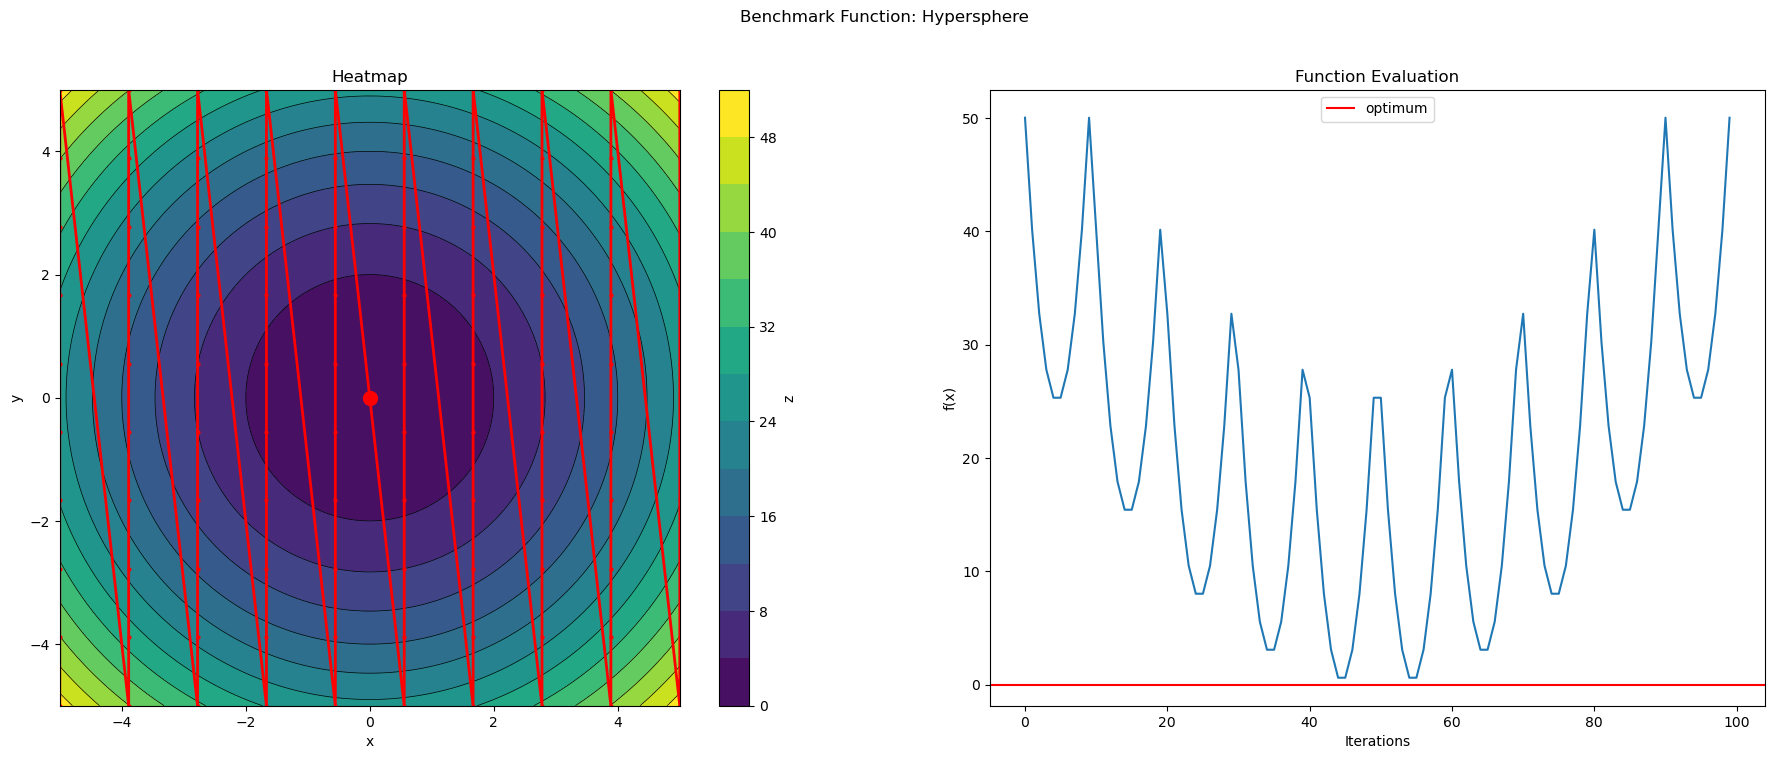
\includegraphics[width=\textwidth]{lab1/imgs/gs_sphere_100.png}
        \caption{Hypersphere function with 100 steps}
    \end{subfigure}
    \begin{subfigure}{0.5\textwidth}
        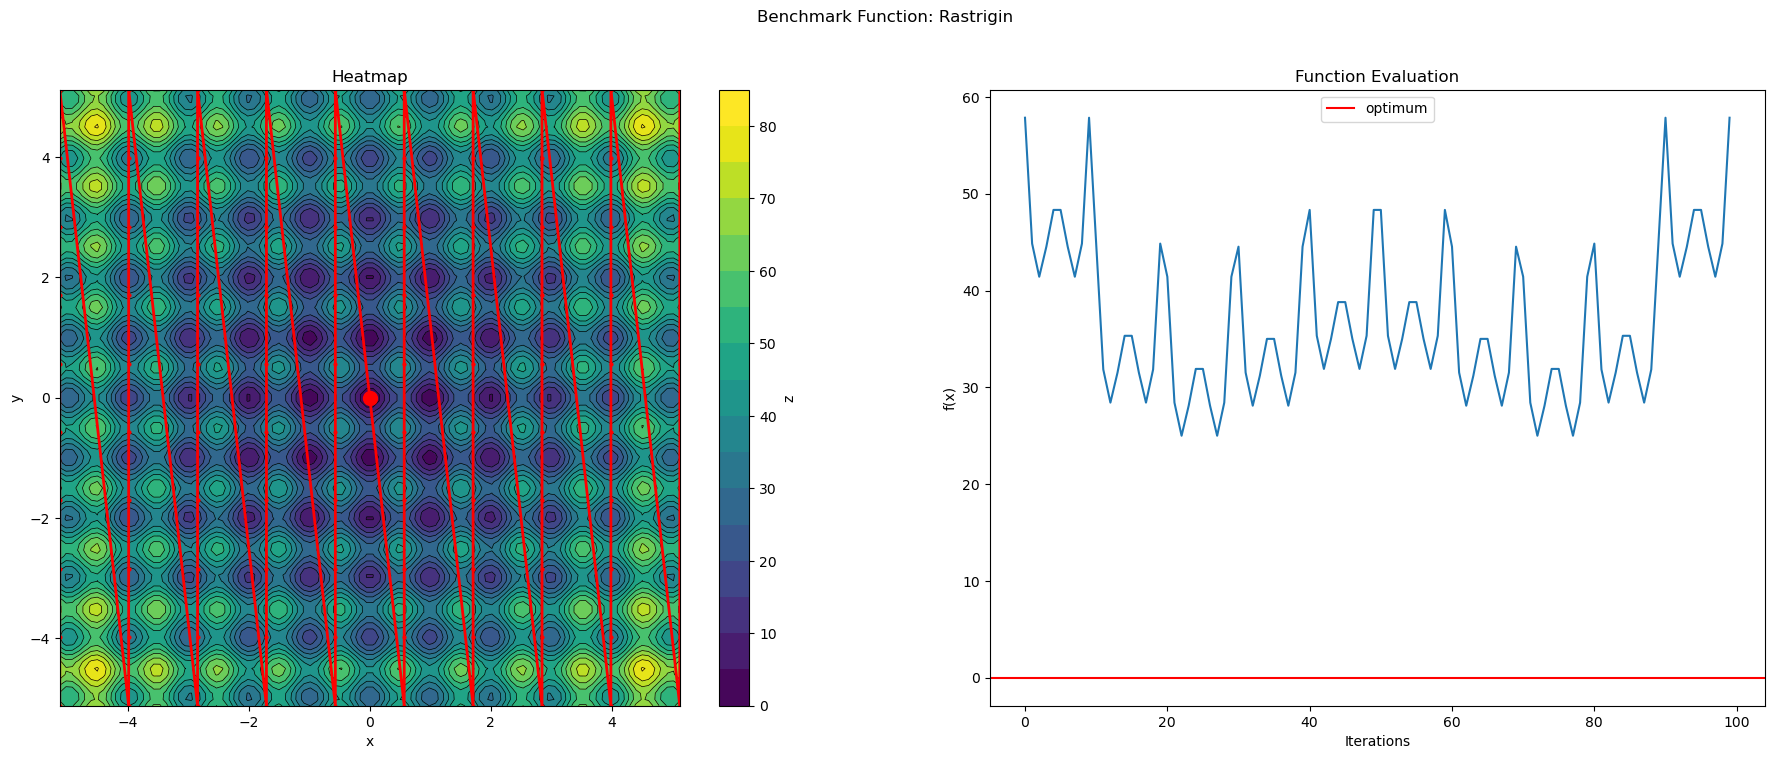
\includegraphics[width=\textwidth]{lab1/imgs/gs_rastrigin_100.png}
        \caption{Rastrigin function with 100 steps}
    \end{subfigure}
    \caption{Comparison between grid search on the Hypersphere and Rastrigin functions}
    \label{fig:gs-100}
\end{figure}

Given that an uniformed search is performed, this means that there is no risk of getting stuck in a local minima but at the same time no information abount the actual shape of the function is used to guide the search. This means that the search is not efficient and the number of steps required to find the global minimum can be very high. At the same it time it can also happen that a higher number of steps doesn't result in an improved solution simply because the discretization of the search space ends up sampling points with a worse objective function. For example we can see this in the example below \ref{fig:gs-ackley} with the Ackley function where 10 steps are able to perfectly find the minimum while 100 steps can't (this is mainly due to the fact the search space is a square and the minimum is exactly in zero so the discretization with 10 steps contains exactly the minimum).

\begin{figure}[H]
    \begin{subfigure}{0.5\textwidth}
        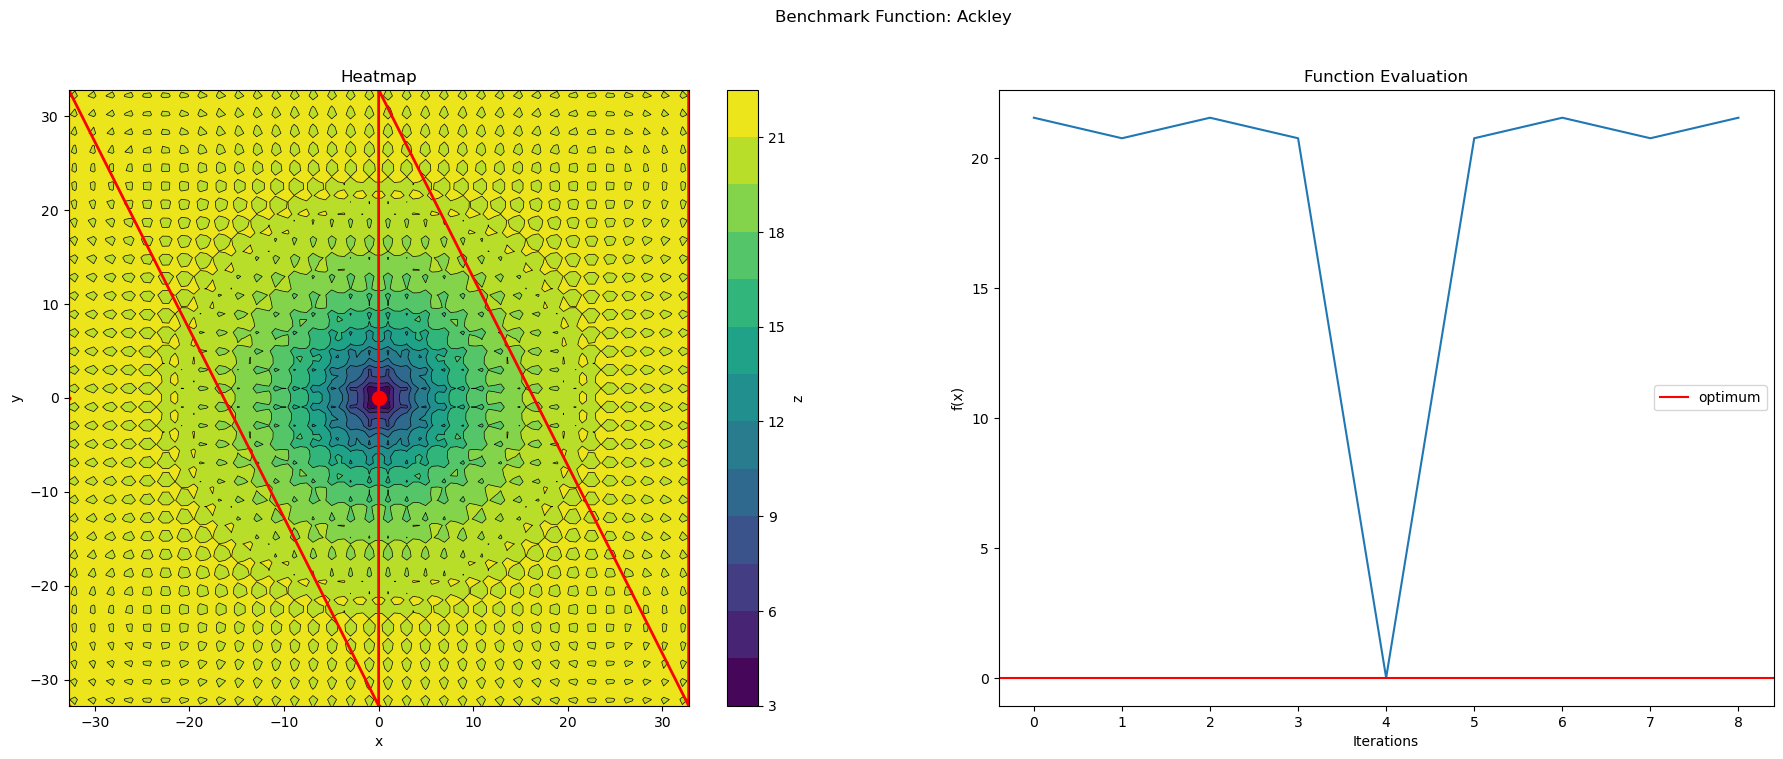
\includegraphics[width=\textwidth]{lab1/imgs/gs_ackley_10.png}
        \caption{Ackley function with 10 steps}
    \end{subfigure}
    \begin{subfigure}{0.5\textwidth}
        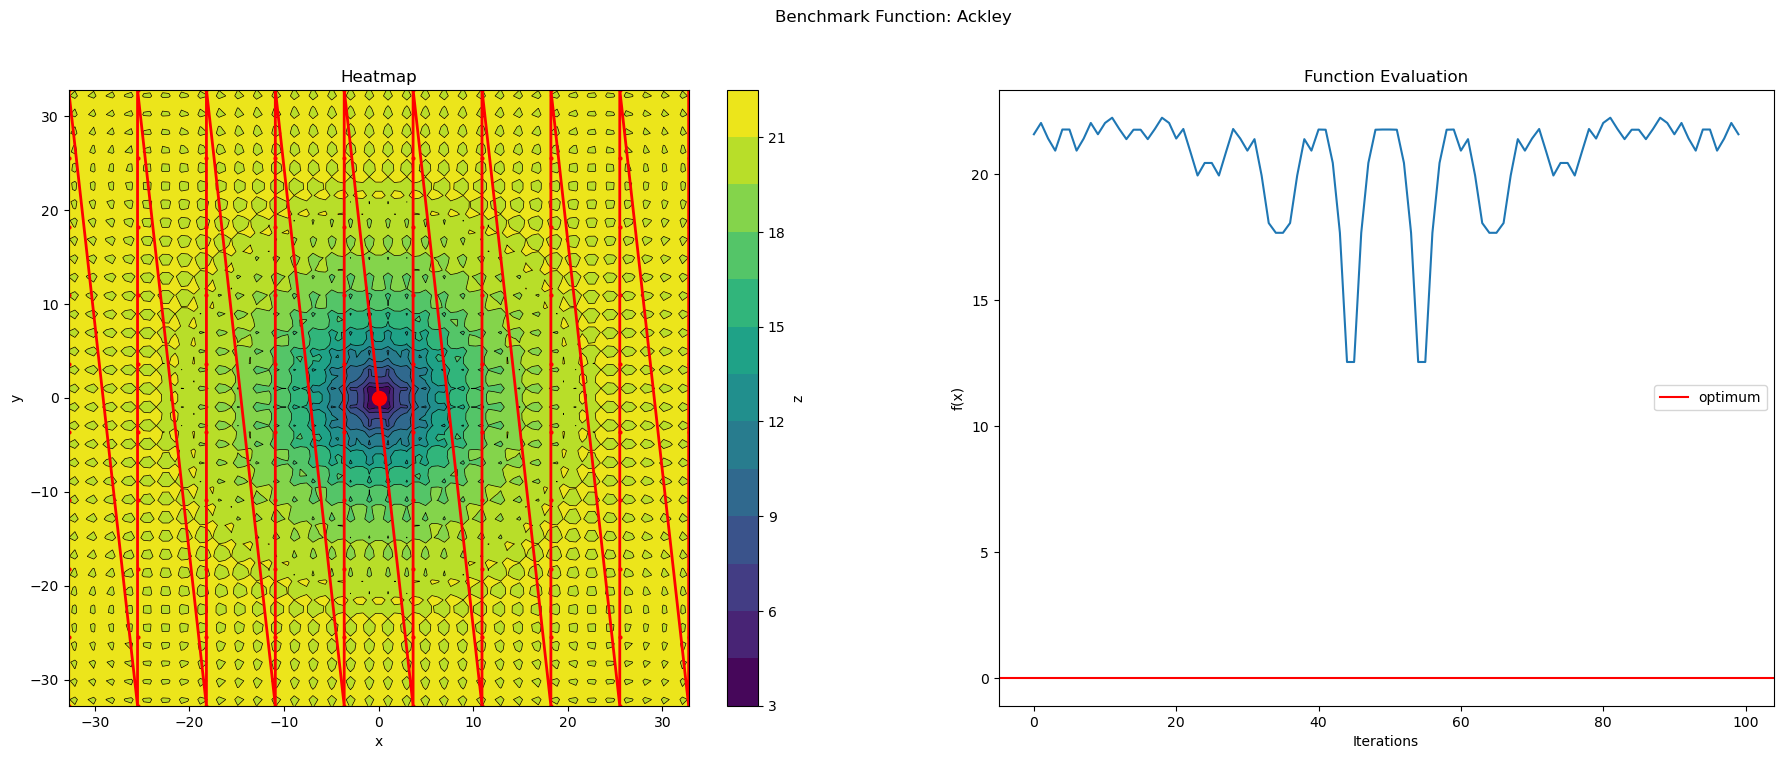
\includegraphics[width=\textwidth]{lab1/imgs/gs_ackley_100.png}
        \caption{Ackley function with 100 steps}
    \end{subfigure}
    \caption{Grid search on the Ackley function}
    \label{fig:gs-ackley}
\end{figure}


\subsection{Random Search}
\label{sec:random-search}
Random search is an uninformed search method that samples the search space randomly.
Given that the samples are taken randomly in the search space, all functions are equally hard to optimize (assuming that all fitness functions are equally computationally hard). For example below \ref{fig:rs-100} we can see different functions, all with 100 samples and see that the results are comparable in terms of the quality of the solution found regarless of function.

\begin{figure}[H]
    \begin{subfigure}{0.5\textwidth}
        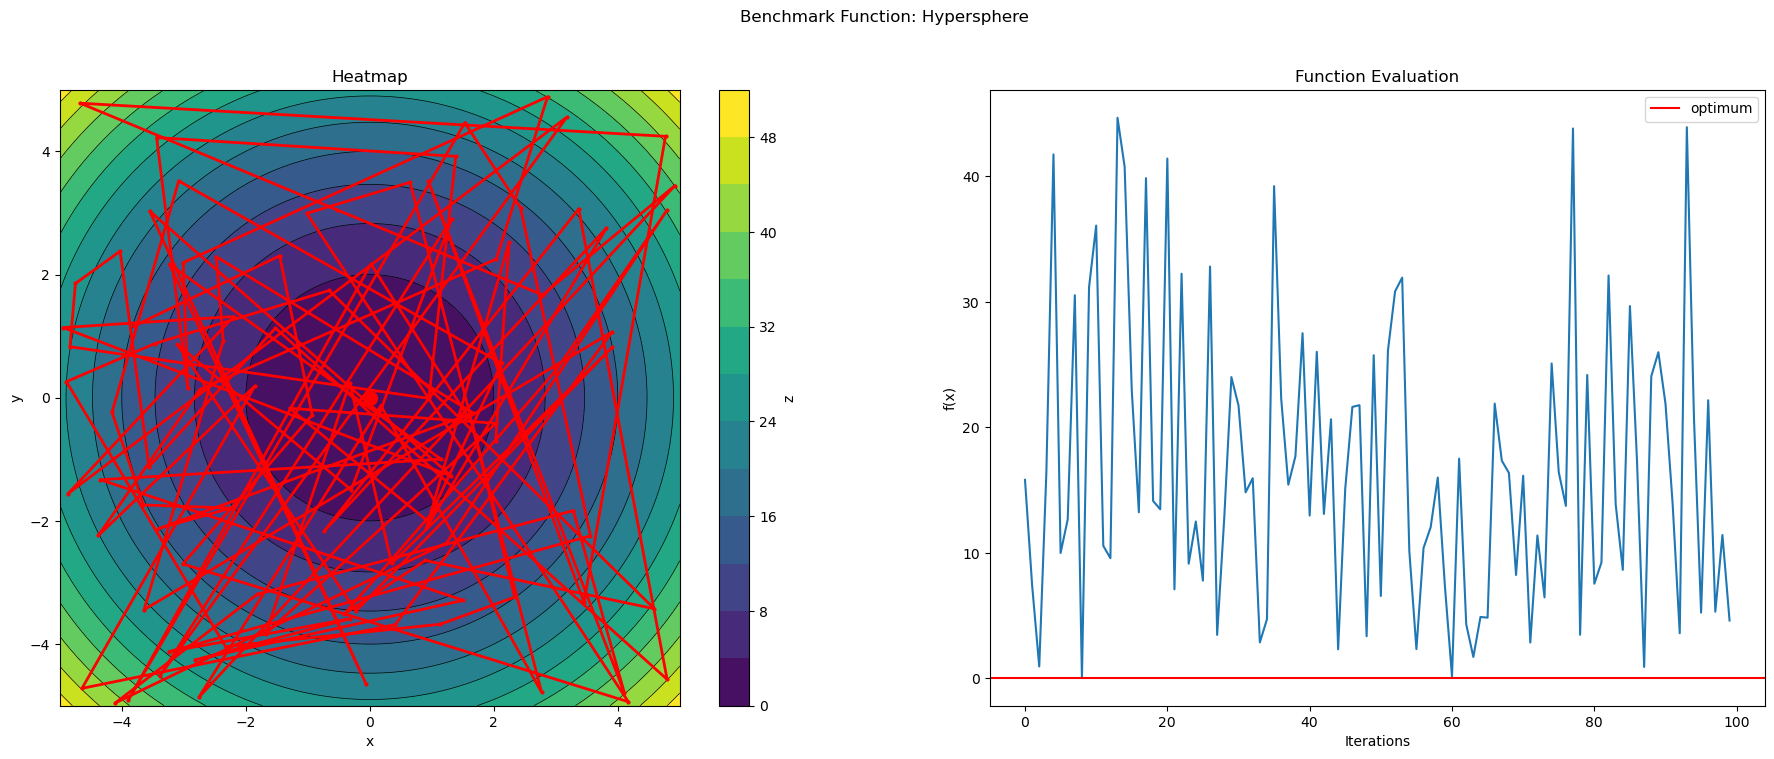
\includegraphics[width=\textwidth]{lab1/imgs/rs_sphere_100.png}
        \caption{Hypersphere}
    \end{subfigure}
    \begin{subfigure}{0.5\textwidth}
        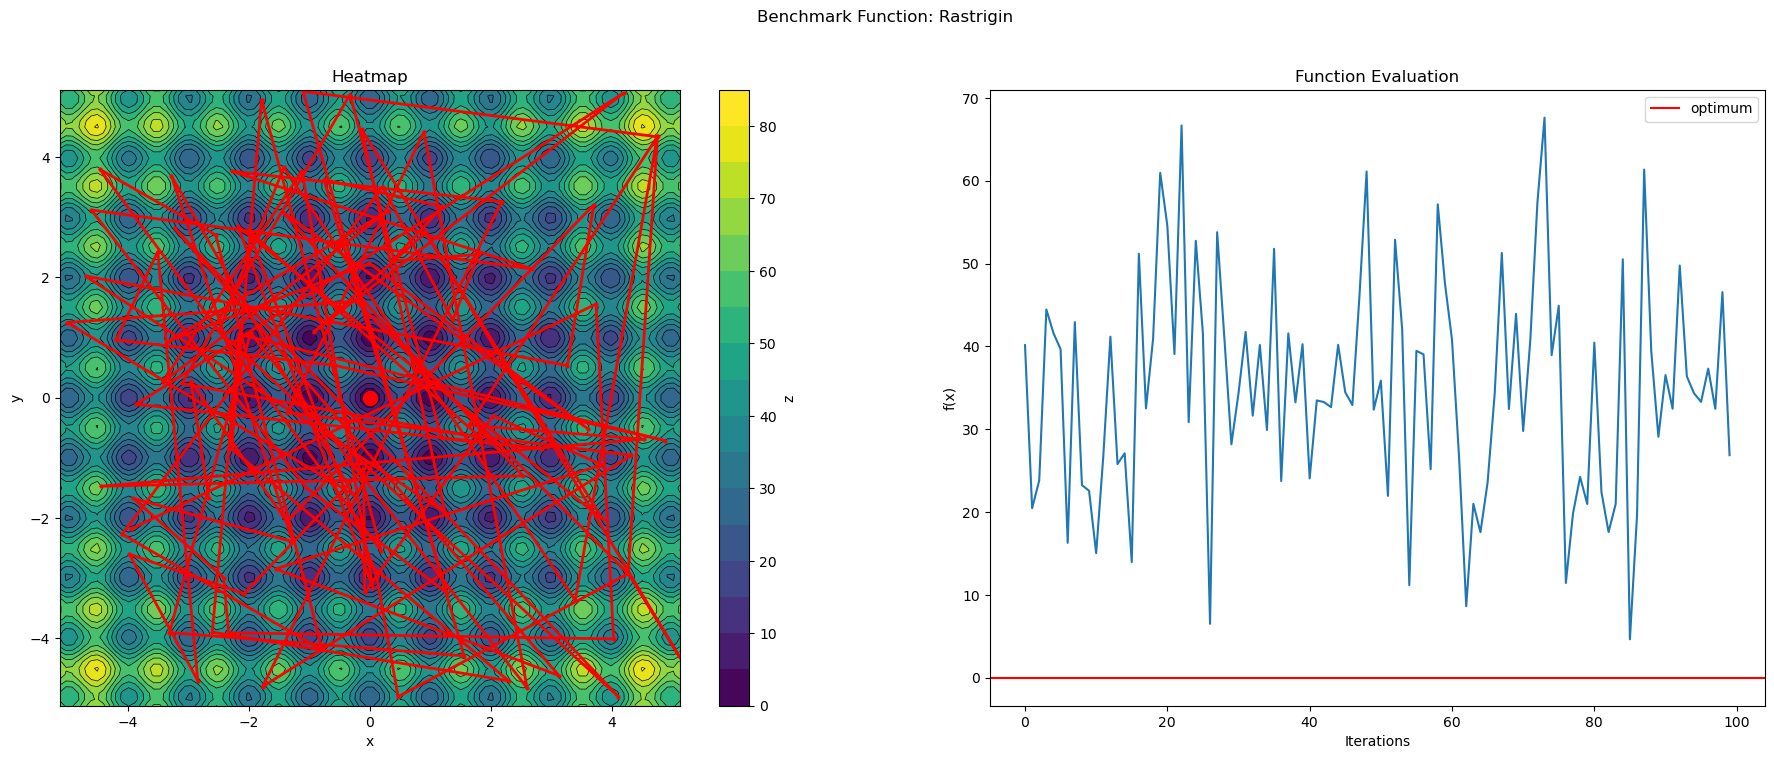
\includegraphics[width=\textwidth]{lab1/imgs/rs_rastrigin_100.png}
        \caption{Rastrigin}
    \end{subfigure} \\
    \begin{subfigure}{\textwidth}
        \centering
        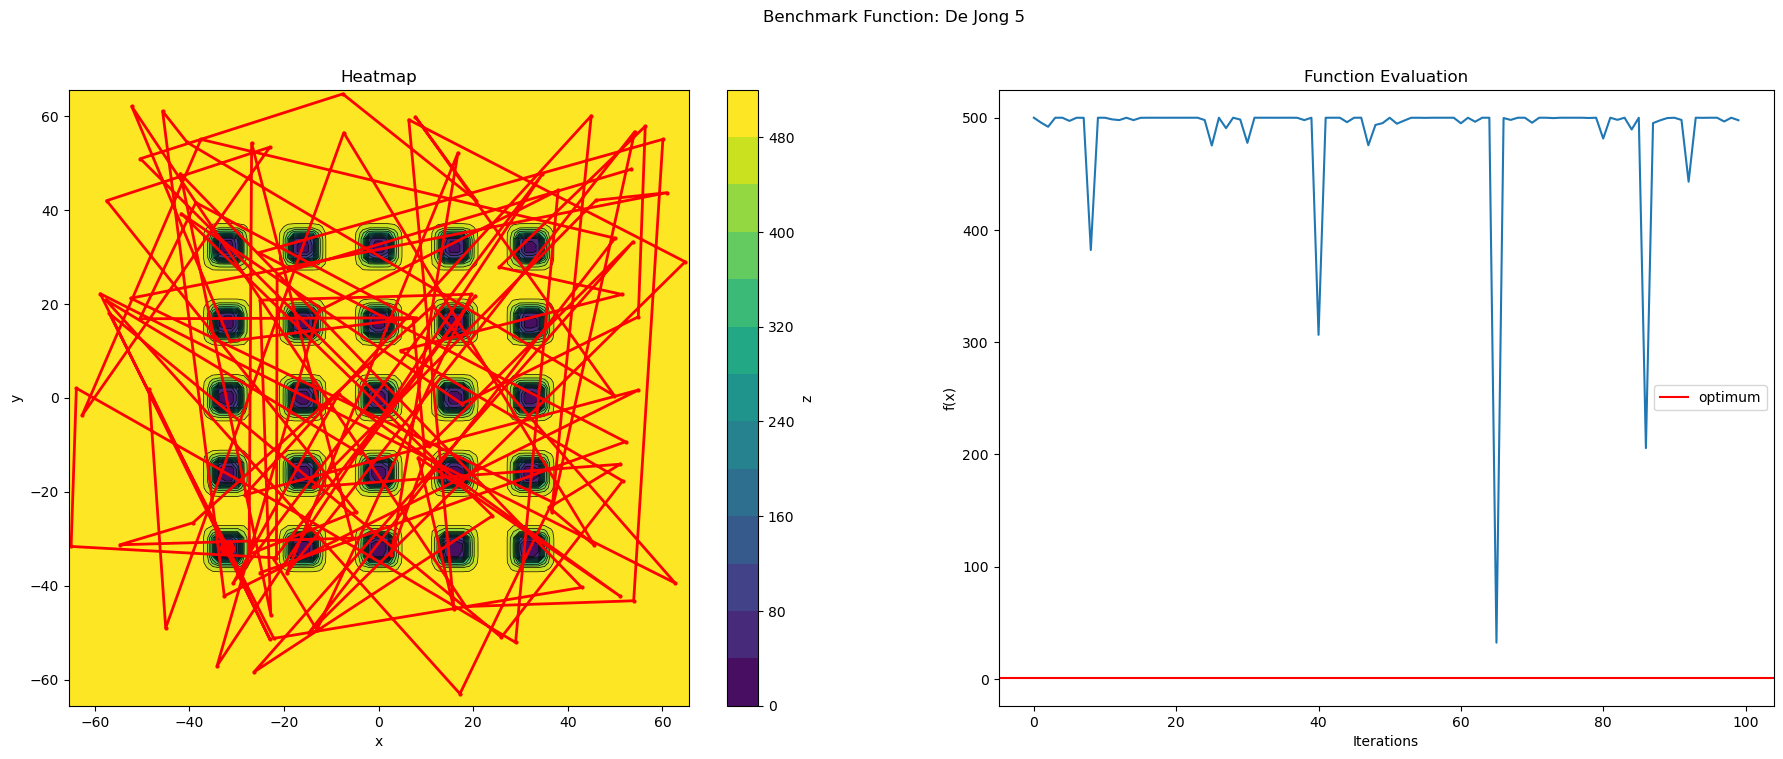
\includegraphics[width=0.5\textwidth]{lab1/imgs/rs_dejong_100.png}
        \caption{DeJong5}
    \end{subfigure}
    \caption{Random search on different functions with 100 samples}
    \label{fig:rs-100}
\end{figure}

\subsection{Powell}
\label{sec:powell}
Powell's method is a conjugate direction method that uses a set of directions to perform a line search. The directions are updated at each iteration to minimize the function. The method is only guaranteed to find a local minimum but in practice it is often able to find the global minimum as well. For example, in the image below \ref{fig:pw} we can see the results of Powell's method on the Rastrigin function, where the method is able to find the global minimum, and the DeJong5 function, where it's not able to, even if the functions are both multimodal.

\begin{figure}[H]
    \begin{subfigure}{0.5\textwidth}
        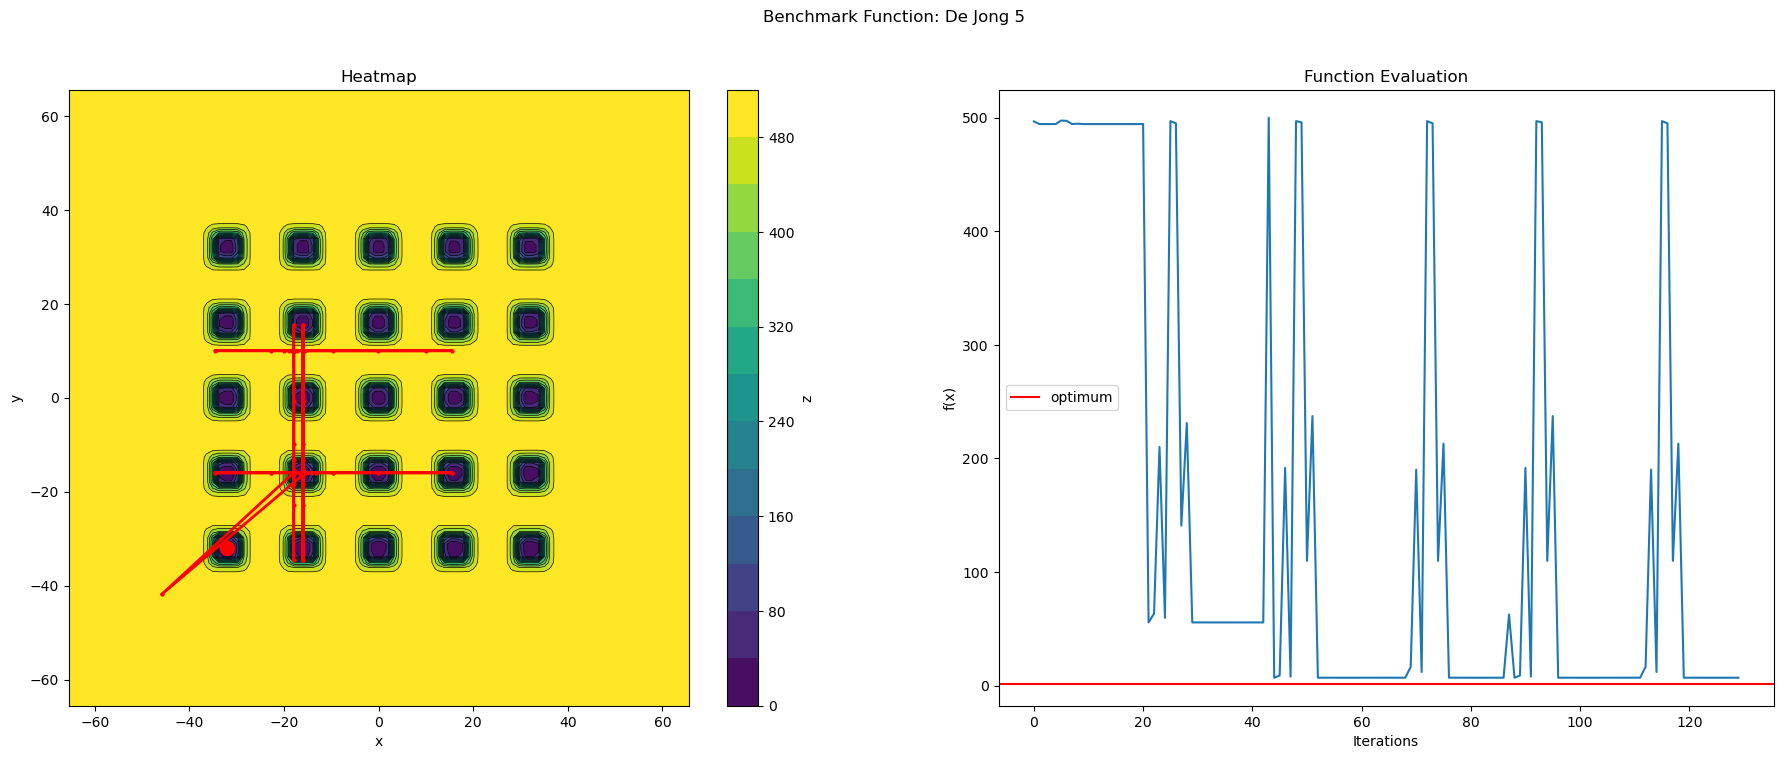
\includegraphics[width=\textwidth]{lab1/imgs/pw_dejong.png}
        \caption{DeJong5}
    \end{subfigure}
    \begin{subfigure}{0.5\textwidth}
        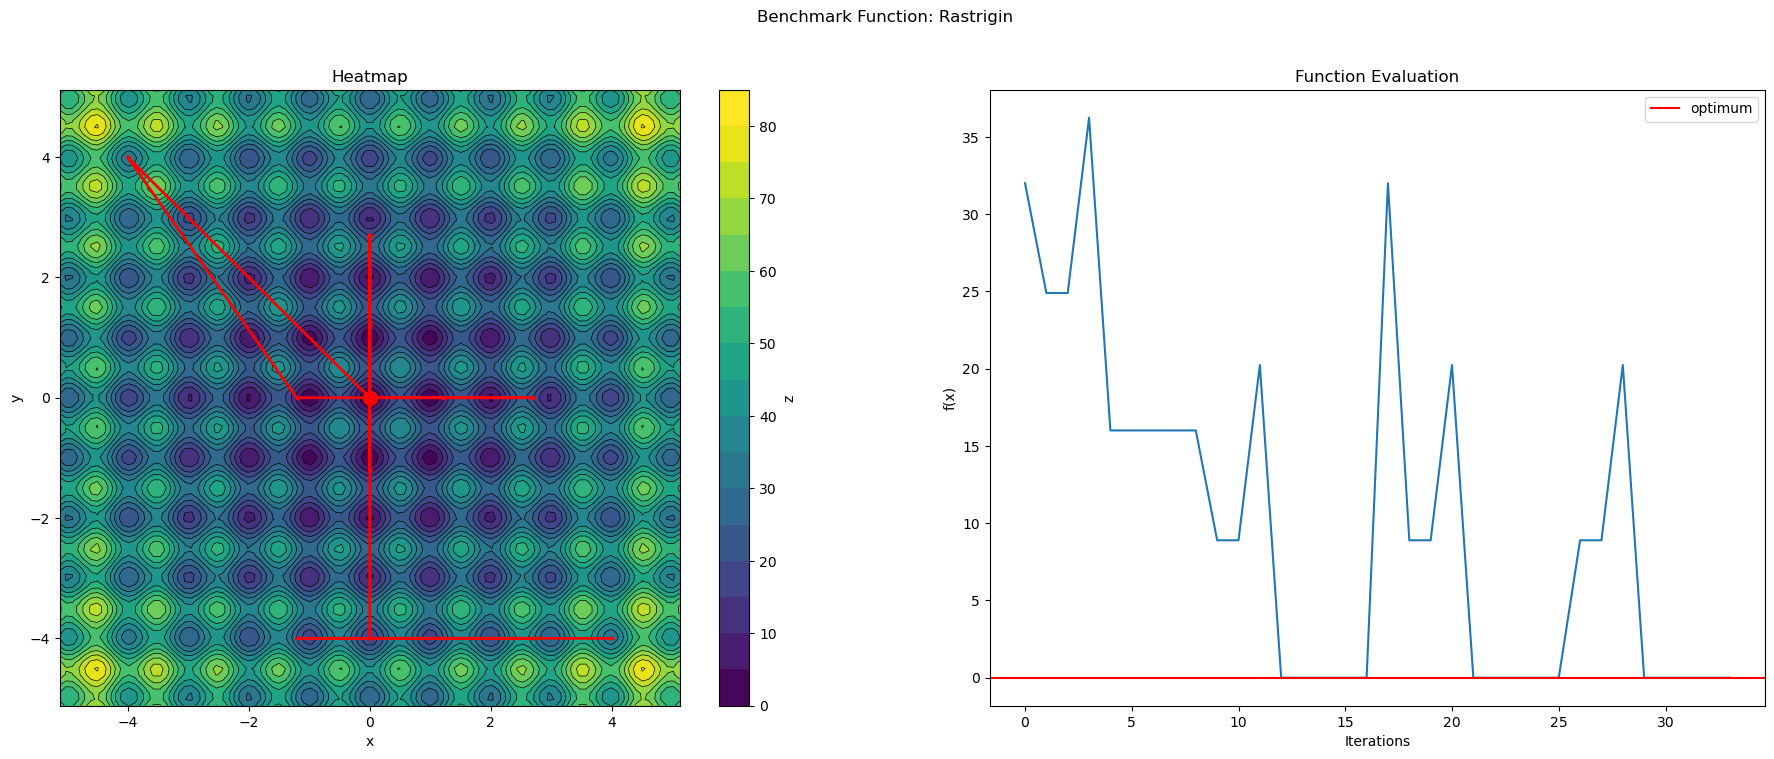
\includegraphics[width=\textwidth]{lab1/imgs/pw_rastrigin.png}
        \caption{Rastrigin}
    \end{subfigure}
    \caption{Powell's method comparison}
    \label{fig:pw}
\end{figure}

Another important aspect of Powell's method is the choice of the initial directions. In the graph below \ref{fig:ackley} we can see that even if the method is able to find the global minimum in both scenarios, the choice of the initial directions has an impact on the number of iterations required to find the minimum.

\begin{figure}[H]
    \begin{subfigure}{0.5\textwidth}
        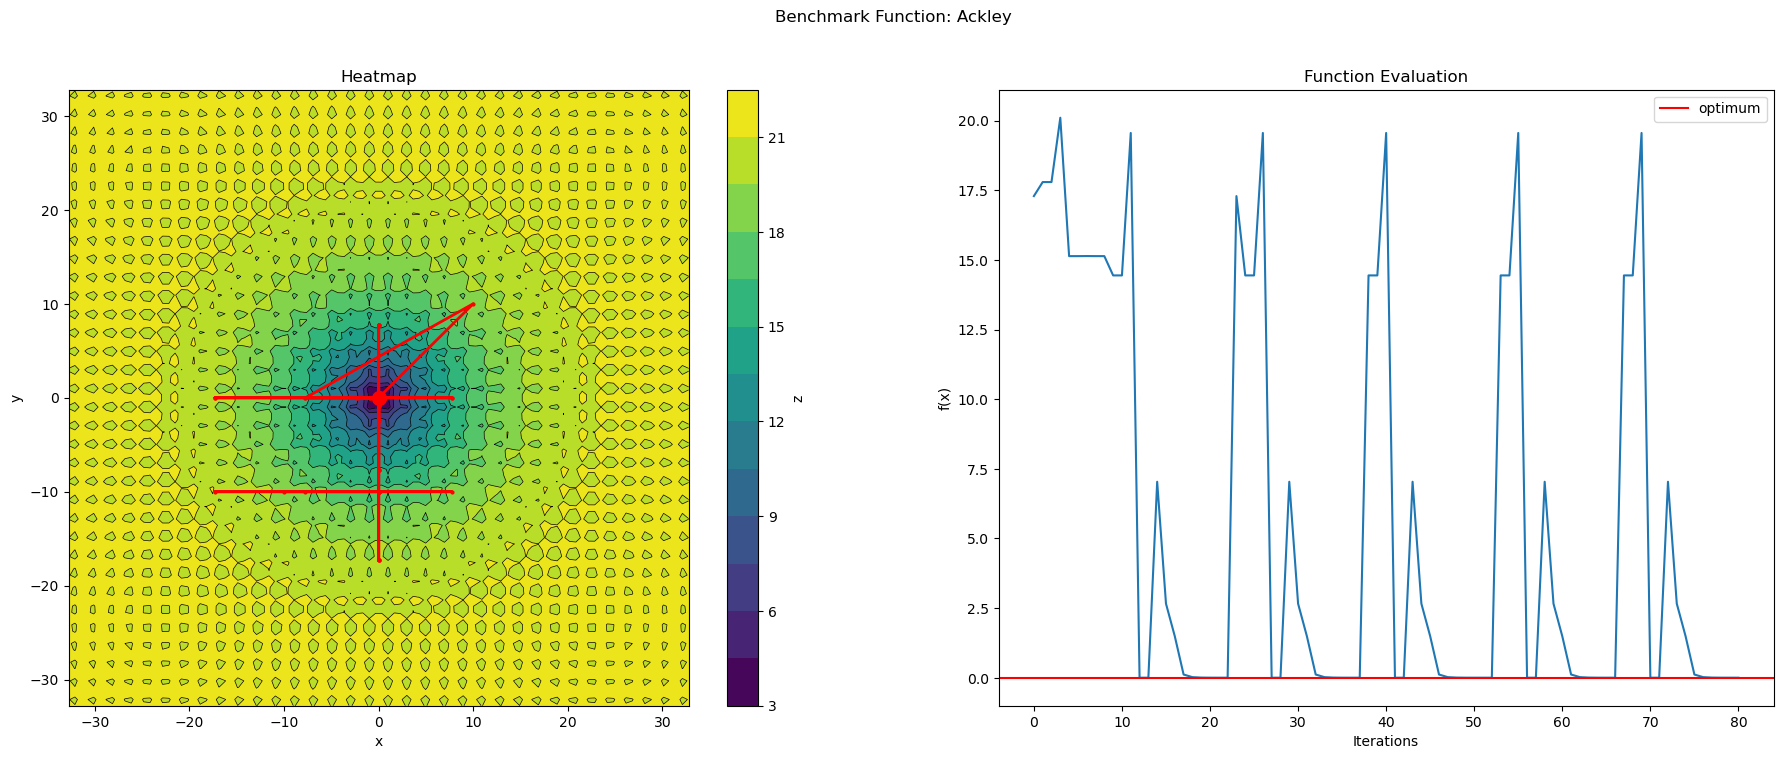
\includegraphics[width=\textwidth]{lab1/imgs/pw_ackley.png}
        \caption{Ackley with directions [[1, 0],[0,1]]}
    \end{subfigure}
    \begin{subfigure}{0.5\textwidth}
        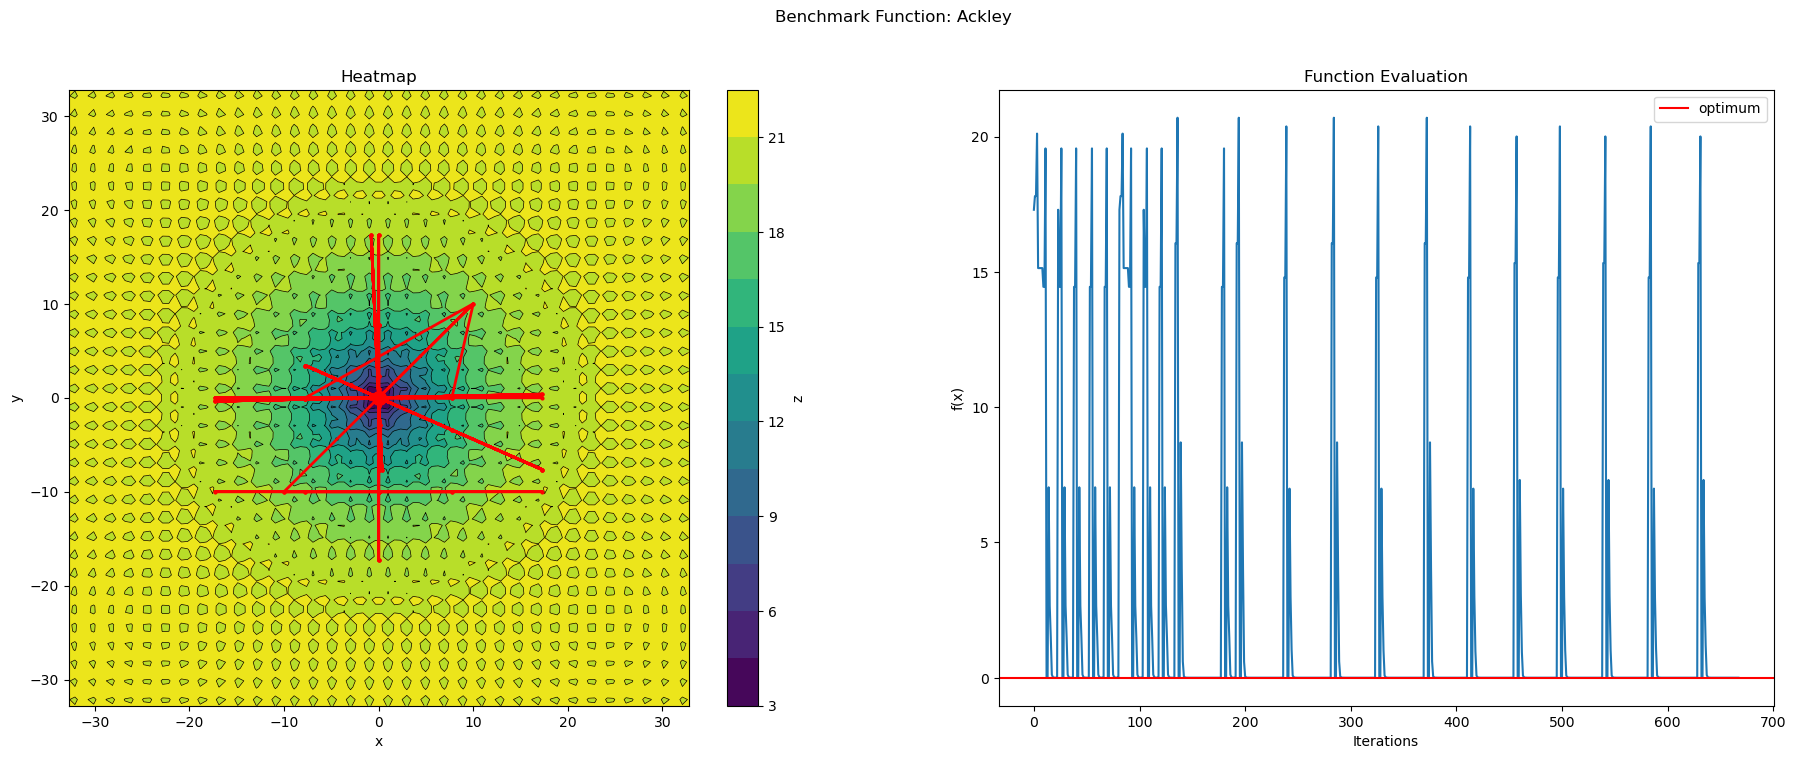
\includegraphics[width=\textwidth]{lab1/imgs/pw_ackley_opposite.png}
        \caption{Ackley with directions [-1,0],[0,-1]}
    \end{subfigure}
    \caption{Powell's method on the Ackley function with different initial directions}
    \label{fig:ackley}
\end{figure}

\subsection{Nelder-Mead}
\label{sec:nelder-mead}
Nelder-Mead is a direct search method that uses a simplex to perform the optimization. Compared to Powell, it's much more likely to get stuck in a local minimum and its performance is dependent on the choice of the initial point. For example below \ref{fig:nm-ackley} we can see the results of Nelder-Mead on the Ackley function where the method is able to converge to the global minimum with the right initial point but not with a different one.
\begin{figure}[H]
    \begin{subfigure}{0.5\textwidth}
        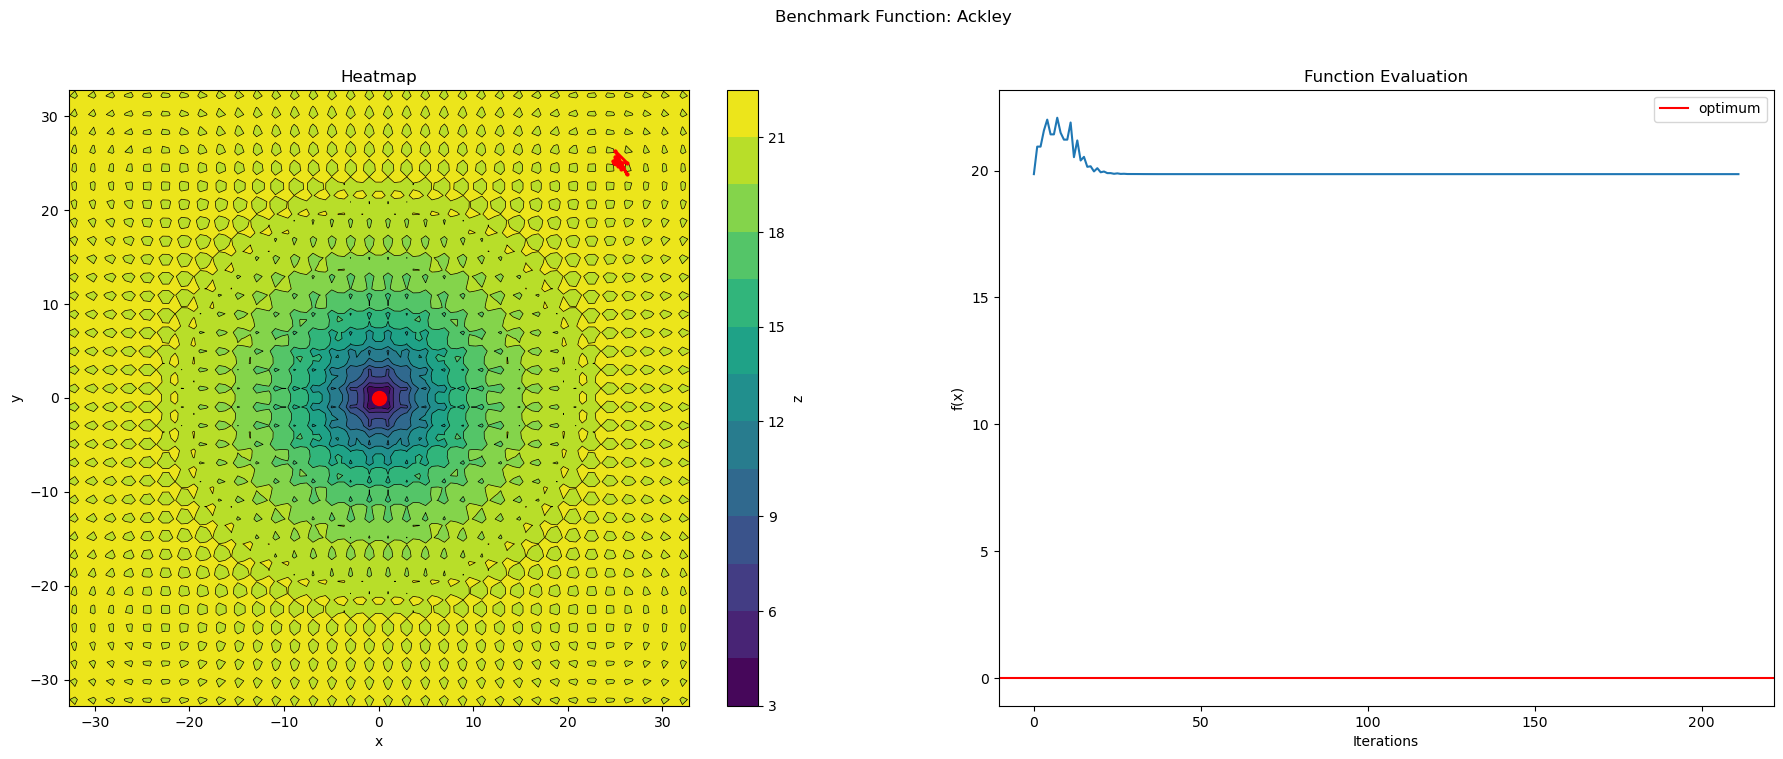
\includegraphics[width=\textwidth]{lab1/imgs/nm_ackley_20.png}
        \caption{Ackley with initial point [20,20]}
    \end{subfigure}
    \begin{subfigure}{0.5\textwidth}
        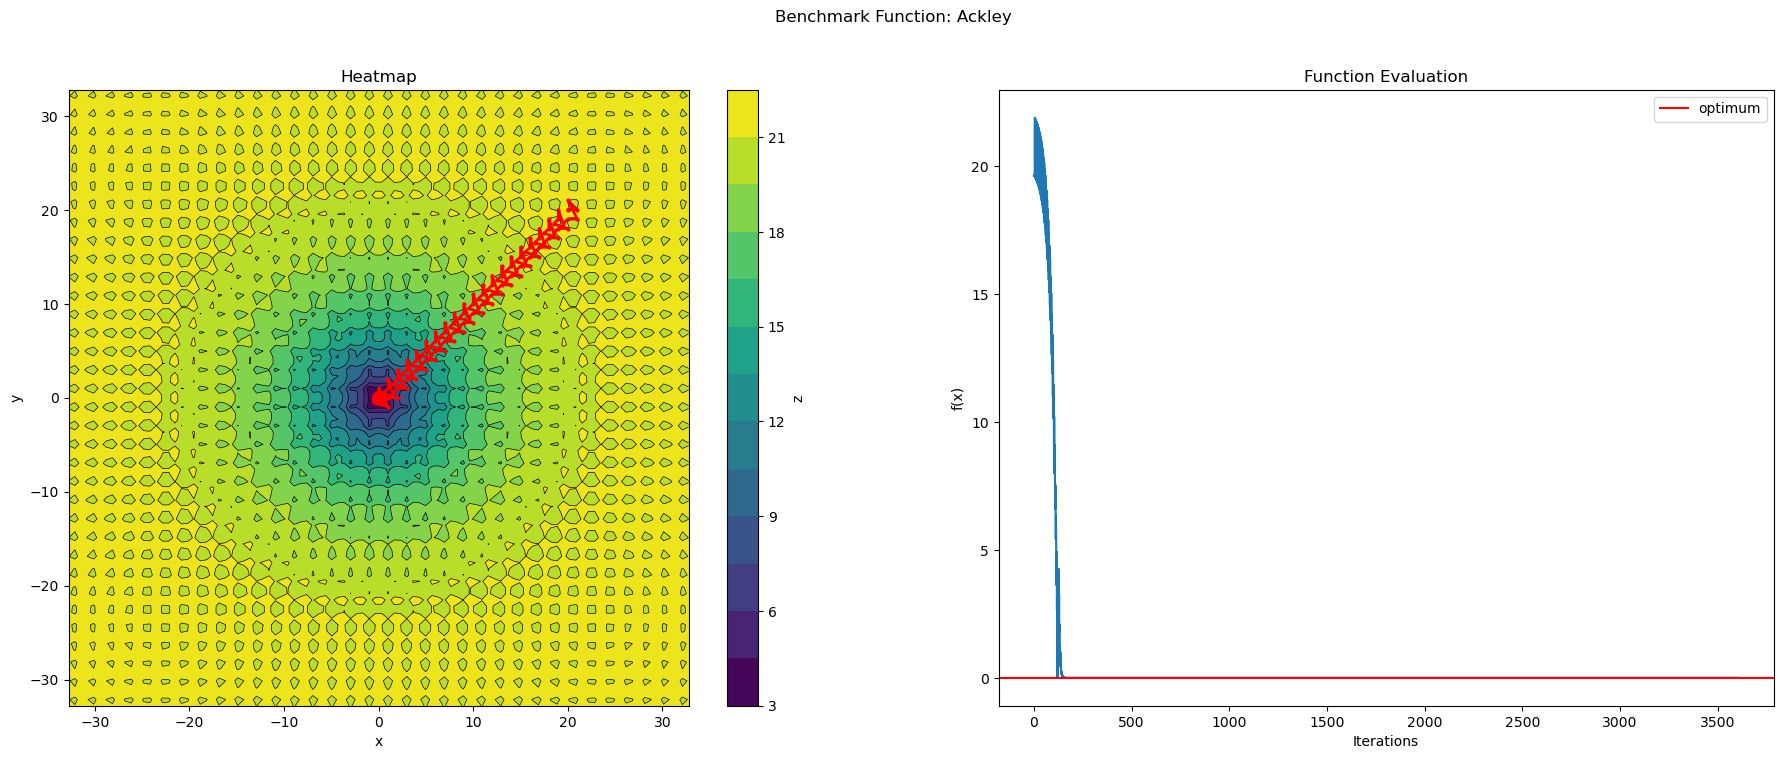
\includegraphics[width=\textwidth]{lab1/imgs/nm_ackley_25.png}
        \caption{Ackley with initial point [25,25]}
    \end{subfigure}
    \caption{Nelder-Mead on the Ackley function with different initial points}
    \label{fig:nm-ackley}
\end{figure}

Below \ref{fig:nm_rosenbrock} we can see the results of Nelder-Mead on the Rosenbrock function and we can see that the algorithms tends to obtain good results in unimodal functions with hard to approximate optima.
\begin{figure}[H]
    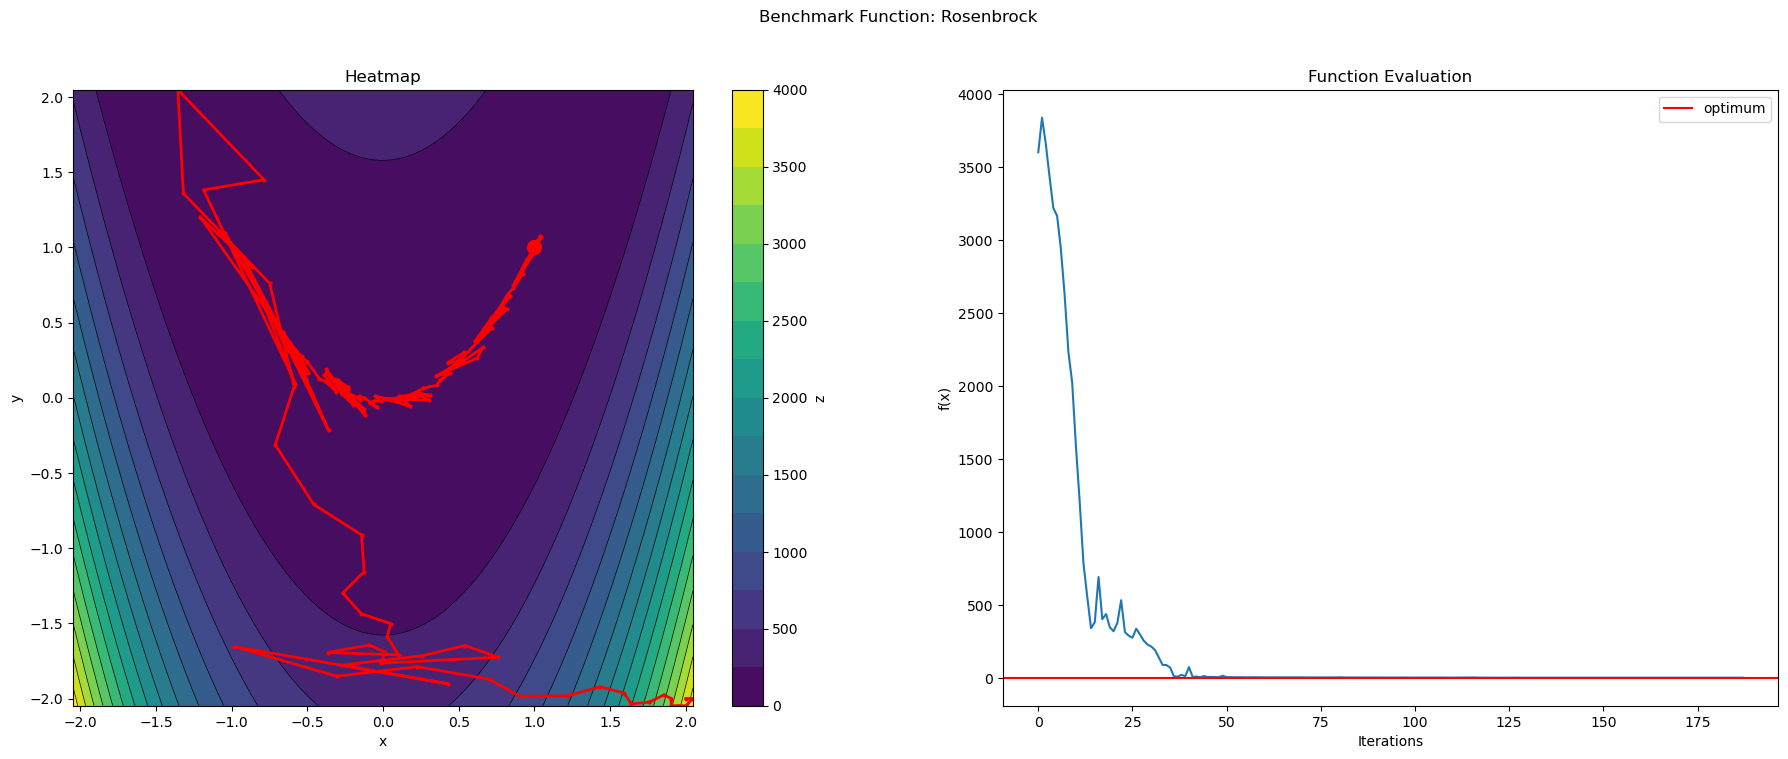
\includegraphics[width=\textwidth]{lab1/imgs/nm_rosenbrock.png}
    \caption{Nelder-Mead on the Rosenbrock function}
    \label{fig:nm_rosenbrock}
\end{figure}
Even on the functions where the method performs well, the number of iterations required is quite high. For example, below \ref{fig:hypersphere-100} we compare the results of the Nelder-Mead and the Powell algorithm on the Hypersphere function, both with 10 iterations.
\begin{figure}[H]
    \begin{subfigure}{0.5\textwidth}
        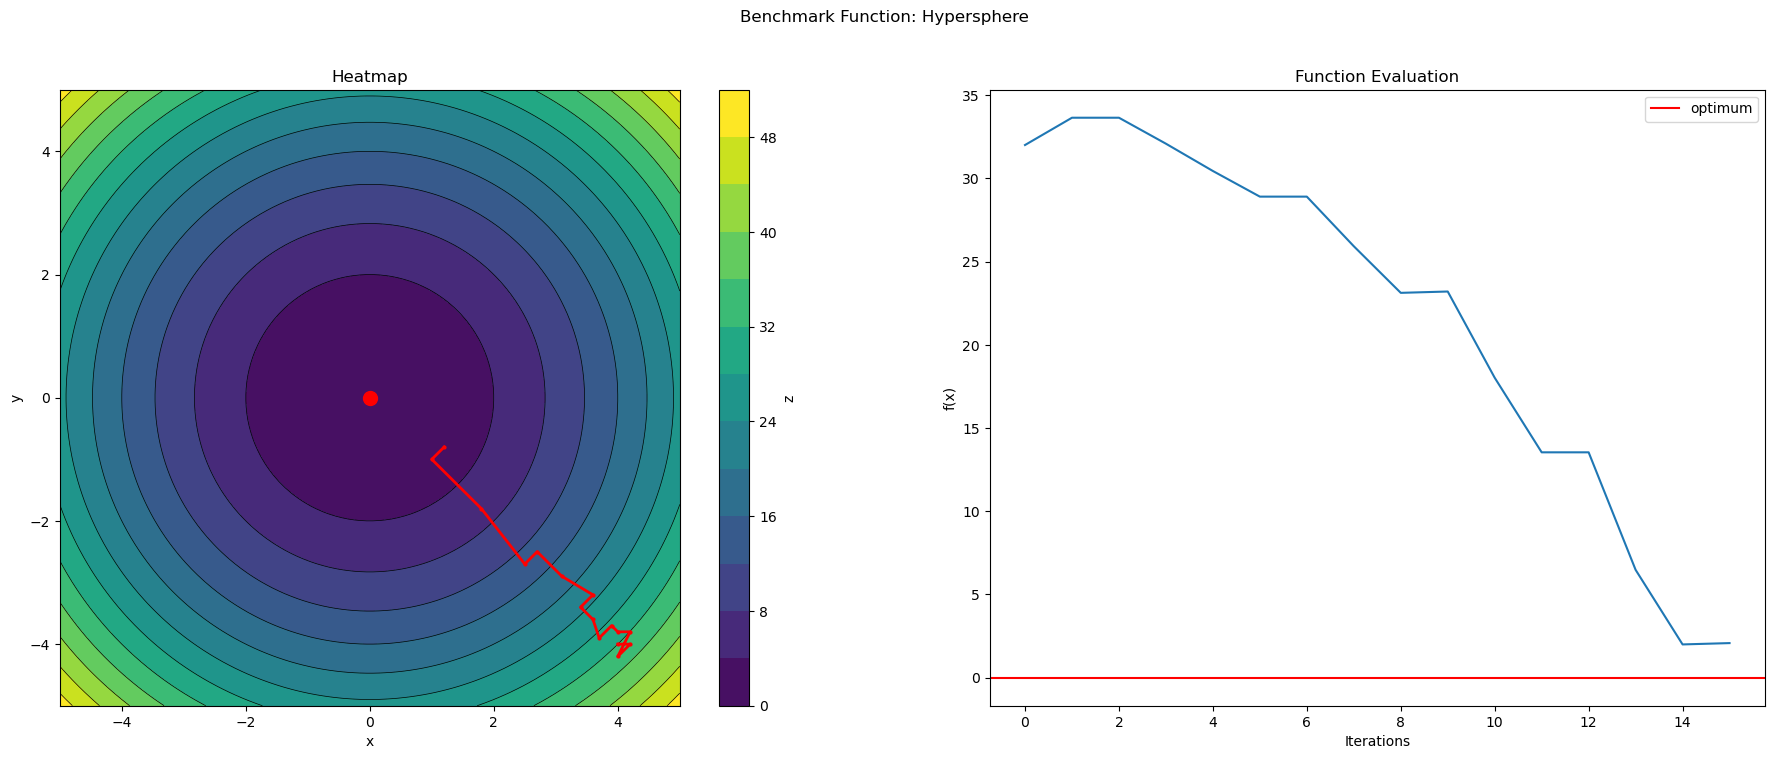
\includegraphics[width=\textwidth]{lab1/imgs/nm_hypersphere_100_iter.png}
        \caption{Nelder-Mead with 10 iterations}
    \end{subfigure}
    \begin{subfigure}{0.5\textwidth}
        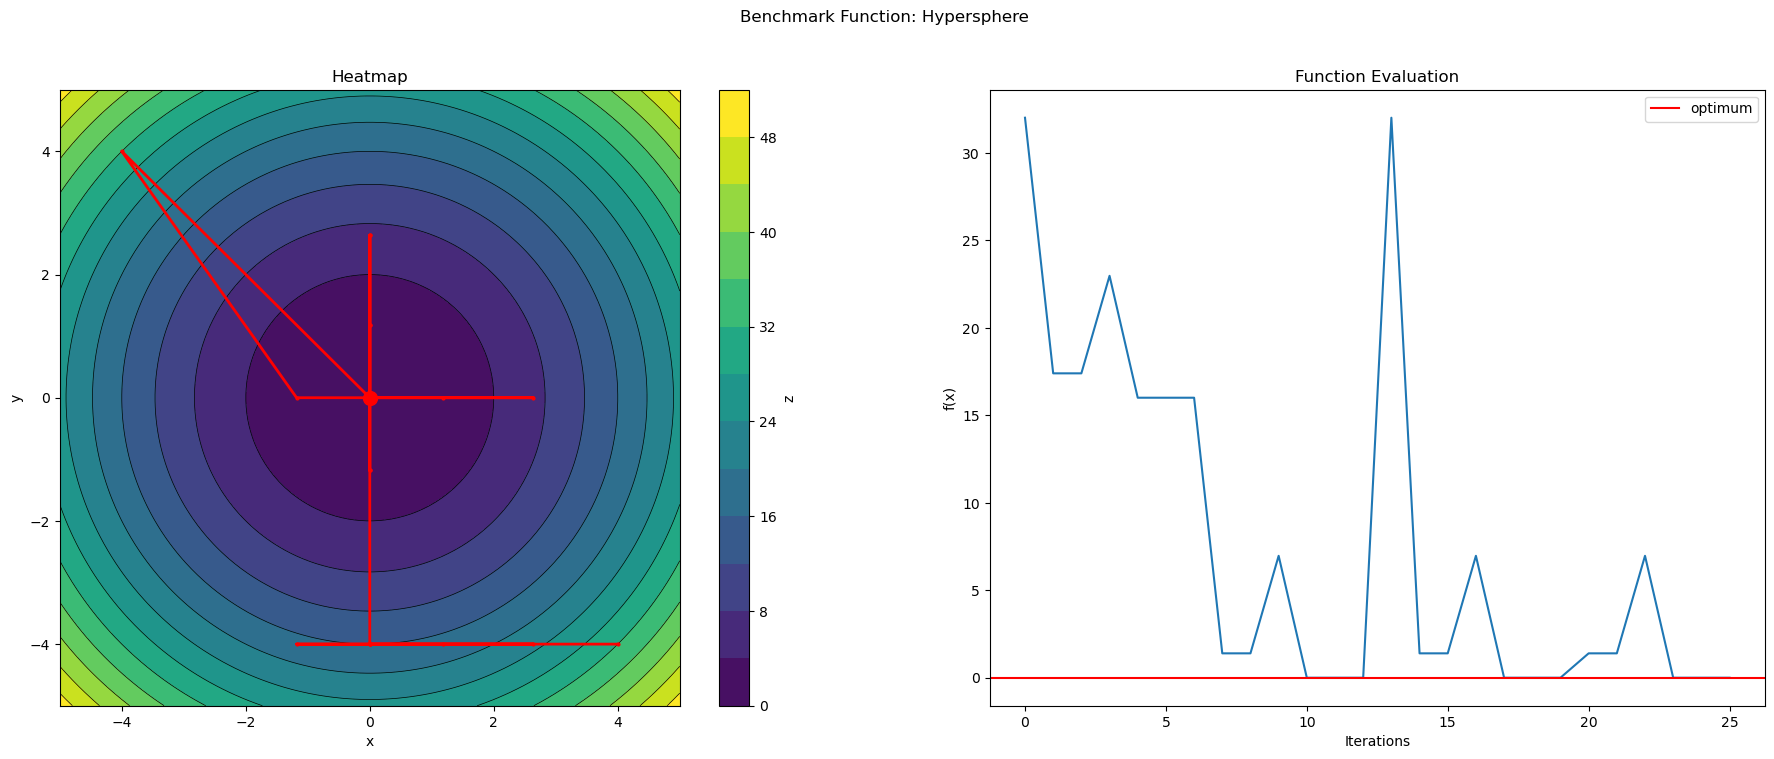
\includegraphics[width=\textwidth]{lab1/imgs/pw_hypersphere_10_iter.png}
        \caption{Powell with 10 iterations}
    \end{subfigure}
    \caption{Nelder-Mead and Powell on the Hypersphere function with 10 iterations}
    \label{fig:hypersphere-100}
\end{figure}
We can see how different methods perform differently on different functions. This is also supported by the No Free Lunch Theorem which states that no optimization algorithm is better than any other when their performance is averaged over all possible functions. This means that the choice of the optimization algorithm is dependent on the specific problem at hand.